\documentclass[]{article}
\usepackage{lmodern}
\usepackage{amssymb,amsmath}
\usepackage{graphicx}
\usepackage{ifxetex,ifluatex}
\usepackage{fixltx2e} % provides \textsubscript
\ifnum 0\ifxetex 1\fi\ifluatex 1\fi=0 % if pdftex
  \usepackage[T1]{fontenc}
  \usepackage[utf8]{inputenc}
\else % if luatex or xelatex
  \ifxetex
    \usepackage{mathspec}
    \usepackage{xltxtra,xunicode}
  \else
    \usepackage{fontspec}
  \fi
  \defaultfontfeatures{Mapping=tex-text,Scale=MatchLowercase}
  \newcommand{\euro}{€}
\fi
% use upquote if available, for straight quotes in verbatim environments
\IfFileExists{upquote.sty}{\usepackage{upquote}}{}
% use microtype if available
\IfFileExists{microtype.sty}{%
\usepackage{microtype}
\UseMicrotypeSet[protrusion]{basicmath} % disable protrusion for tt fonts
}{}
\ifxetex
  \usepackage[setpagesize=false, % page size defined by xetex
              unicode=false, % unicode breaks when used with xetex
              xetex]{hyperref}
\else
  \usepackage[unicode=true]{hyperref}
\fi
\hypersetup{breaklinks=true,
            bookmarks=true,
            pdfauthor={},
            pdftitle={},
            colorlinks=true,
            citecolor=blue,
            urlcolor=blue,
            linkcolor=magenta,
            pdfborder={0 0 0}}
\urlstyle{same}  % don't use monospace font for urls
\setlength{\parindent}{0pt}
\setlength{\parskip}{6pt plus 2pt minus 1pt}
\setlength{\emergencystretch}{3em}  % prevent overfull lines
\providecommand{\tightlist}{%
  \setlength{\itemsep}{0pt}\setlength{\parskip}{0pt}}
\setcounter{secnumdepth}{0}

\date{}

% Redefines (sub)paragraphs to behave more like sections
\ifx\paragraph\undefined\else
\let\oldparagraph\paragraph
\renewcommand{\paragraph}[1]{\oldparagraph{#1}\mbox{}}
\fi
\ifx\subparagraph\undefined\else
\let\oldsubparagraph\subparagraph
\renewcommand{\subparagraph}[1]{\oldsubparagraph{#1}\mbox{}}
\fi

\begin{document}

\section{Goal}\label{goal}

\emph{\textbf{In this chapter,}} \\
* We will learn how to threshold images. \\
* We will see: \textbf{cv2.threshold()}

\section{Theory}\label{theory}

Thresholding is the simplest method of image segmentation. From a
grayscale image, thresholding can be used to create binary images. Here,
the matter is straight forward. If pixel value is greater than a
threshold value, it is assigned one value (may be white), else it is
assigned another value (may be black). The function used is
cv2.threshold. First argument is the source image, which should be a
grayscale image. Second argument is the threshold value which is used to
classify the pixel values. Third argument is the maxVal which represents
the value to be given if pixel value is more than (sometimes less than)
the threshold value. OpenCV provides different styles of thresholding
and it is decided by the fourth parameter of the function. Different
types are:\\
• \texttt{cv2.THRESH\_BINARY}\\
• \texttt{cv2.THRESH\_BINARY\_INV}\\
• \texttt{cv2.THRESH\_TOZERO}\\
• \texttt{cv2.THRESH\_TRUNC}\\
• \texttt{cv2.THRESH\_TOZERO\_INV}

How to use the function?\\
The function takes three inputs. First is the source image(img), second
argument is the threshold value which is used to classify the pixel
values. Third argument is the Max\_value which represents the value to
be given if pixel value is more than (sometimes less than) the threshold
value.
\begin{verbatim}
	cv2.threshold(img, 127, 255, cv2.THRESH_BINARY)
\end{verbatim}

\section{Code}\label{code}

Below we will see an example on how to use thresholding to images.
Consider the sunflower image below:
\begin{figure}[h]
	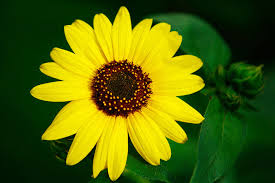
\includegraphics{sun.jpg}
\end{figure}

\newpage
\begin{verbatim}
'''
**********************************************************************************
*                                                                                *
*                   IMAGE PROCESSING ( THRESHOLDING OPERATION )                  *
*                                                                                *
*                                                                                *
*  TEAM MEMBERS : NIHARIKA JAYANTHI, DHEERAJ KAMATH                              *
*                                                                                *
*  MENTOR : SANAM SHAKYA                                                         *
*                                                                                *
*  FILENAME : THRESHOLDING.PY                                                    *
*                                                                                *
*  THEME : DEVELOP MODULES FOR IMAGE PROCESSING AND ROBOT LOCALISATION           * 
*          USING MARKERS                                                         *
*                                                                                *
*  FUNCTIONS : cv3.threshold(), cv2.cvtColor(), cv2.imread()                     *
*                                                                                *
*  GLOBAL VARIABLES : NONE                                                       *
*                                                                                *
**********************************************************************************
'''

########################

import cv2                  #Import OpenCV
import numpy as np          #Import Numpy

########################

'''
Initialisation of the camera is done by the function cv2.imread
'''
img = cv2.imread('sun.jpg')

'''
To convert the image into grayscale we use the command
cv2.cvtColor(img, cv2.COLOR_BGR2GRAY)
'''
gray = cv2.cvtColor(img, cv2.COLOR_BGR2GRAY)

##########################################################################################
'''
* FUNCTION NAME : ret,thresh = cv2.threshold(img, Min_value,Max_value,cv2.THRESH_BINARY)
* INPUT         : Input is a source image which should be in grayscale.
* OUTPUT        : A thresholded image will  be displayed.
* LOGIC         : The function takes three inputs. First is the source image(img),
                  second argument is the threshold value which is used to classify the 
                  pixel values.
                  Third argument is the Max_value which represents the value to be given 
                  if pixel value is more than (sometimes less than) the threshold value.
* EXAMPLE CALL  : ret,thresh = cv2.threshold( img, 0, 255, cv2.THRESH_BINARY)
* ADITIONAL INFO: Different types are:
                  cv2.THRESH_BINARY
                  cv2.THRESH_BINARY_INV
                  cv2.THRESH_TRUNC
                  cv2.THRESH_TOZERO
                  cv2.THRESH_TOZERO_INV
'''
#####################################################################
ret, thresh  = cv2.threshold(gray,127,255,cv2.THRESH_BINARY)
ret, thresh1 = cv2.threshold(gray,127,255,cv2.THRESH_BINARY_INV)
ret, thresh2 = cv2.threshold(gray,127,255,cv2.THRESH_TRUNC)
ret, thresh3 = cv2.threshold(gray,127,255,cv2.THRESH_TOZERO)
ret, thresh4 = cv2.threshold(gray,127,255,cv2.THRESH_TOZERO_INV)

'''
* To display the image we use the function cv2.imshow()
'''
cv2.imshow("Thresh", thresh)
cv2.imshow("Thresh1", thresh1)
cv2.imshow("Thresh2", thresh2)
cv2.imshow("Thresh3", thresh3)
cv2.imshow("Thresh4", thresh4)

'''
* cv2.waitKey() - Waits for the user to click any key.
* cv2.destroyAllWindows() - Closes all output tabs.
'''
cv2.waitKey(0)
cv2.destroyAllWindows()
\end{verbatim}

Output Images:

\begin{enumerate}
\def\labelenumi{\arabic{enumi})}
\item Thresh Binary\\
  \begin{figure}[h]
  	
\includegraphics{Threshbinary.jpg}
  \end{figure}
\newpage
\item Thresh Binary Inverse \\
  \begin{figure}[h]
  	
\includegraphics{ThreshBinaryInv.jpg}
  \end{figure}
\item Thresh Trunc\\
  \begin{figure}[h]
  	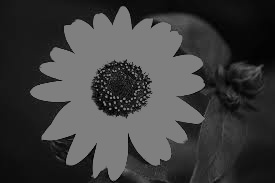
\includegraphics{ThreshTrunc.jpg}
  \end{figure}
\newpage
\item Thresh To Zero\\
  \begin{figure}[h]
  	\includegraphics{ThreshToZero.jpg}
  \end{figure}
\item Thresh To Zero Inv\\
  \begin{figure}[h]
  	\includegraphics{ThreshToZeroInv.jpg}
  \end{figure}
\end{enumerate}

\newpage
\section{Additional Resources}\label{additional-resources}

\begin{enumerate}
\def\labelenumi{\arabic{enumi})}
\tightlist
\item
  \url{http://docs.opencv.org/doc/tutorials/imgproc/threshold/threshold.html}
\end{enumerate}

\section{Excercises}\label{excercises}

\end{document}
